\chapter{Практическая часть}

Ниже представленны листинги программы:

\lstset{language=python}
\begin{lstlisting}[caption=Исходные данные]
K0 = 0.4
KN = 0.1
alpha0 = 0.05
alphaN = 0.01
l = 10
T0 = 300
R = 0.5
F0 = 50
h = 1e-3
\end{lstlisting}

\lstset{language=python}
\begin{lstlisting}[caption=Параметры для краевых условий]
b = (KN * l) / (KN - K0)
a = - K0 * b
d = (alphaN * l) / (alphaN - alpha0)
c = - alpha0 * d
\end{lstlisting}

\lstset{language=python}
\begin{lstlisting}[caption=Коэффициенты теплопроводности и теплоотдачи]
def k(x):
    return a / (x - b)

def alpha(x):
    return c / (x - d)
\end{lstlisting}

\lstset{language=python}
\begin{lstlisting}[caption=Выполнение замены]
def p(x):
    return 2 * alpha(x) / R

def f(x):
    return 2 * alpha(x) * T0 / R
\end{lstlisting}

\lstset{language=python}
\begin{lstlisting}[caption=Простая аппроксимация]
def x_plus_half(x):
    return (k(x) + k(x + h)) / 2

def x_minus_half(x):
    return (k(x) + k(x - h)) / 2
\end{lstlisting}

\lstset{language=python}
\begin{lstlisting}[caption=Разностная схема]
def A(x):
    return x_plus_half(x) / h

def C(x):
    return x_minus_half(x) / h

def B(x):
    return A(x) + C(x) + p(x) * h

def D(x):
    return f(x) * h
\end{lstlisting}

\lstset{language=python}
\begin{lstlisting}[caption=Краевые условия при x = 0]
K0 = x_plus_half(0) + h * h * (p(0) + p(h)) / 16 + h * h * p(0) / 4
M0 = -(x_plus_half(0) - h * h * (p(0) + p(h)) / 16)
P0 = h * F0 + h * h / 4 * ((f(0) + f(h)) / 2 + f(0))
\end{lstlisting}
\lstset{language=python}
\begin{lstlisting}[caption=Краевые условия при x = N]
KN = -x_minus_half(l) / h - alphaN - p(l) * h / 4 - (p(l) + p(l - h)) * h / 16
MN = x_minus_half(l) / h - (p(l) + p(l - h)) * h / 16
PN = -(alphaN * T0 + ((f(l) + f(l - h)) / 2 + f(l)) * h / 4)
\end{lstlisting}

\lstset{language=python}
\begin{lstlisting}[caption=Метод прогонки]
def run():
    eps = [0, -M0 / K0]
    eta = [0, P0 / K0]

    x = h
    n = 1
    while (x + h < l):
        eps.append(C(x) / (B(x) - A(x) * eps[n]))
        eta.append((D(x) + A(x) * eta[n]) / (B(x) - A(x) * eps[n]))
        n += 1
        x += h

    t = [0] * (n + 1)
    t[n] = (PN - MN * eta[n]) / (KN + MN * eps[n])

    for i in range(n - 1, -1, -1):
        t[i] = eps[i + 1] * t[i + 1] + eta[i + 1]

    return t
\end{lstlisting}

На изображениях ниже представлены скриншот работы программы:
\begin{enumerate}
    \item График зависимости температуры $T(x)$ от координаты $x$ при заданных выше параметрах:
\begin{figure}[H]
    \centering
    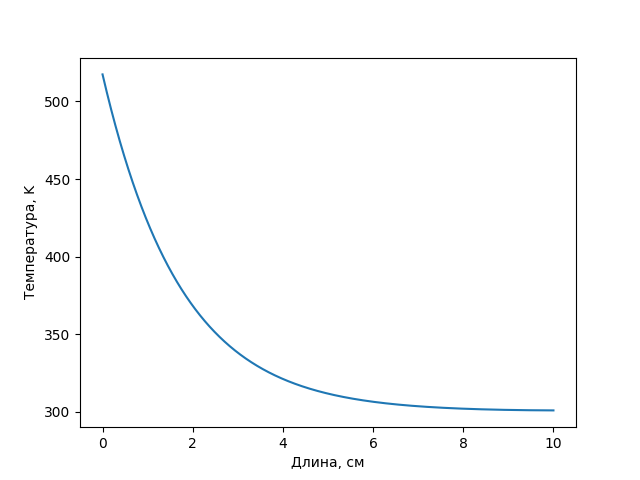
\includegraphics[scale=0.9]{data/pdf/Figure_1.png}
\end{figure}

\item График зависимости $T(x)$ при $F_0$ = -10.
\begin{figure}[H]
    \centering
    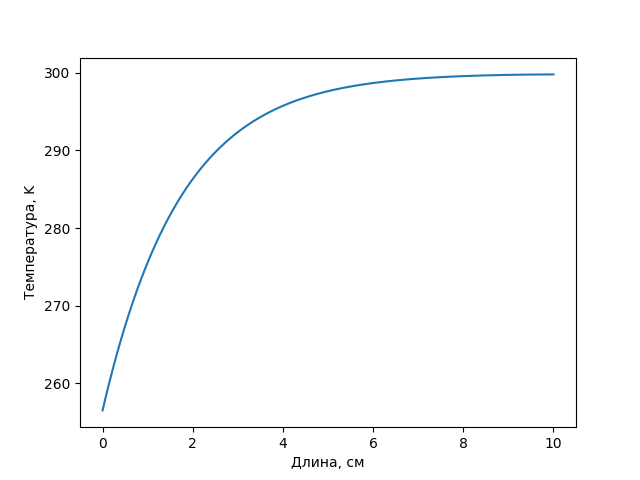
\includegraphics[scale=0.9]{data/pdf/Figure_2.png}
\end{figure}

\item График зависимости  при увеличенных значениях (например, в 3 раза).
\begin{figure}[H]
    \centering
    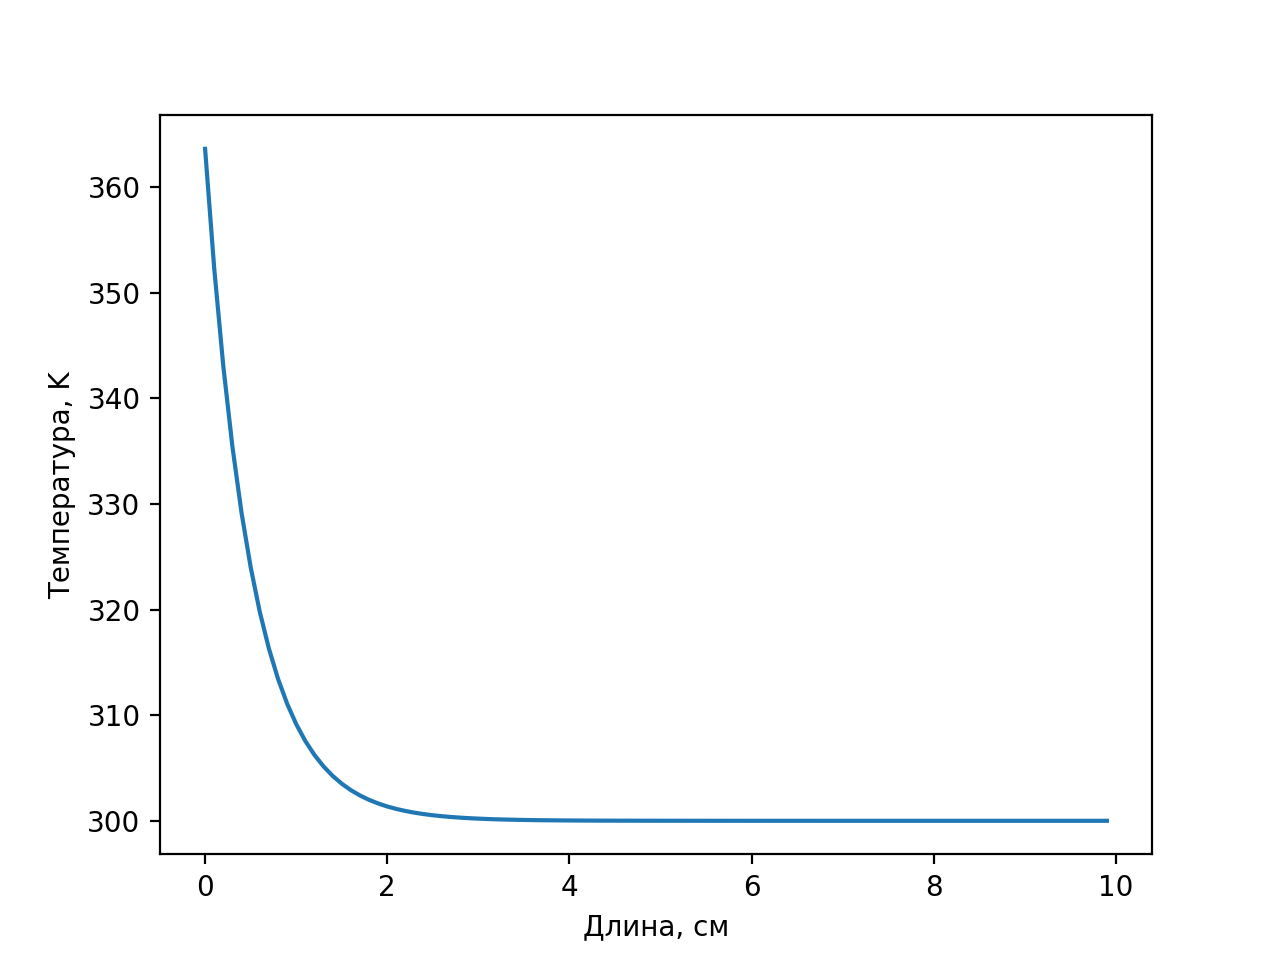
\includegraphics[scale=0.9]{data/pdf/graph3.png}
\end{figure}
\textbf{Справка.}
При увеличении теплосъема и неизменном потоке  уровень температур  должен снижаться, а градиент увеличиваться.

\item График зависимости $T(x)$ при $F_0 = 0$.
Так как используемая библиотека приближает график по осям таким образом, чтобы границами графика являлись минимальные и максимальные значения, на этом графике прямой не видно.
\begin{figure}[H]
    \centering
    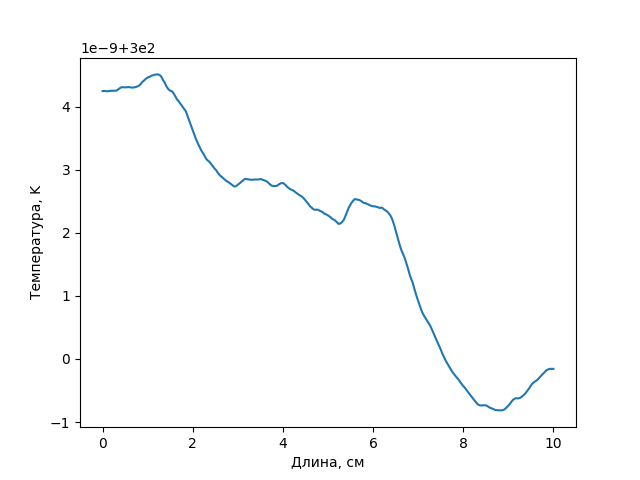
\includegraphics[scale=0.9]{data/pdf/Figure_5.png}
\end{figure}

Для получения желаемого графика выведем значения, полученные программой, и посторим график по ним:
\begin{figure}[H]
    \centering
    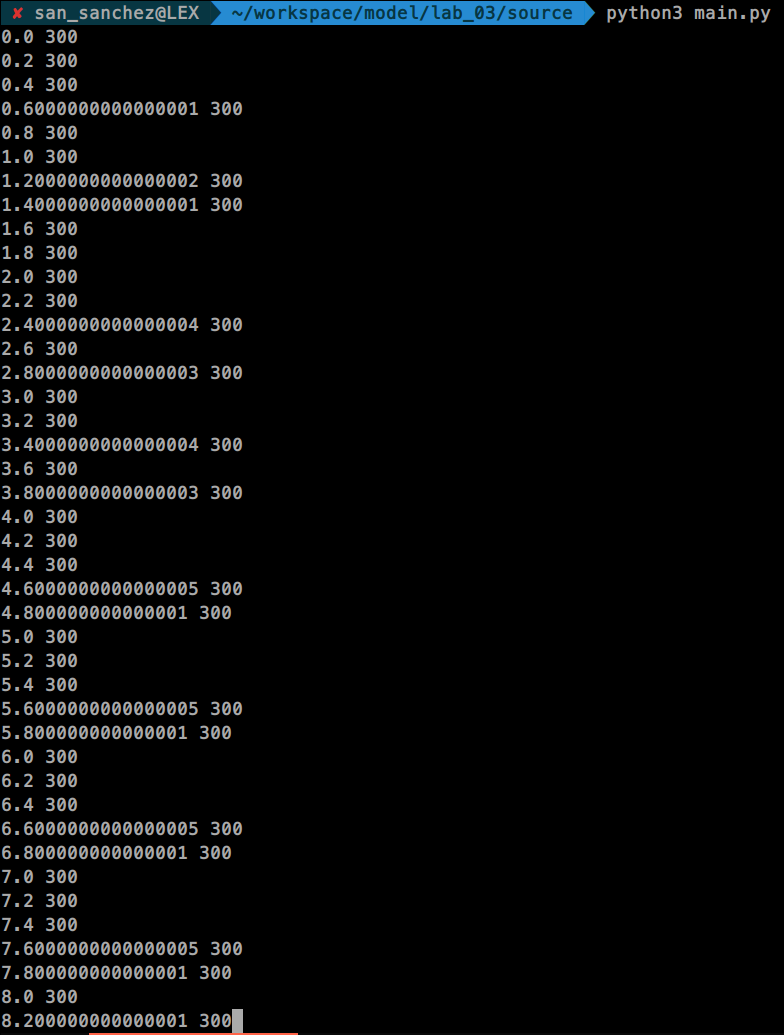
\includegraphics[scale=0.6]{data/pdf/res.png}
\end{figure}
\begin{figure}[H]
    \centering
    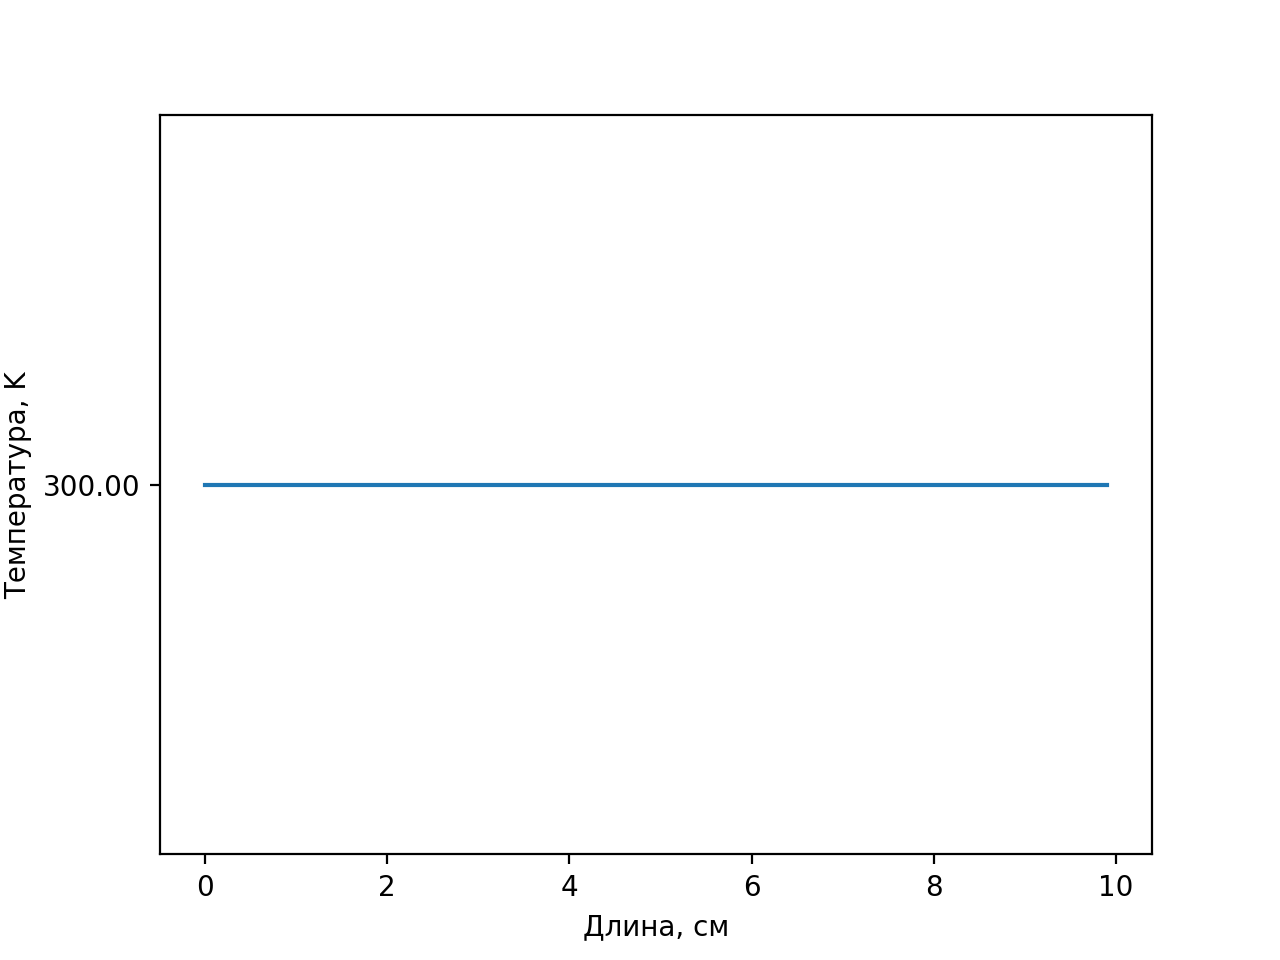
\includegraphics[scale=0.9]{data/pdf/graph4.png}
	\caption{Вывод программы}
\end{figure}


\textbf{Справка.}
В данных условиях тепловое нагружение отсутствует, причин для нагрева нет, температура стержня должна быть равна температуре окружающей среды $T_0$  (разумеется, с некоторой погрешностью, определяемой приближенным характером вычислений).
\end{enumerate}

